%TODO
% Fotos Team
% Überarbeiten
% Sprint Backlog Bild verwenden? (zitieren)
% Product Owner Quelle kein Autor

\section{Projektmanagement und Organisation}
\label{sec:ProjUOrg}

\subsection{Team} %Fotos fehlen noch
\label{sec:Team}
	\subsubsection*{Dario Wagner}
		Verantwortlich für: 
		\begin{itemize}
			\item Parser
			\item iCal
		\end{itemize}
	\subsubsection*{Marcel Stering}
		Verantwortlich für: 
		\begin{itemize}
			\item Security
			\item Webseite
		\end{itemize}
	\subsubsection*{Matthias Franz}
		Verwantwortlich für: 
		\begin{itemize}
			\item iCal
			\item Datenbank
			\item Projektleitung
		\end{itemize}				

\subsection{Auftraggeber - Intact Systems}
\label{sec:Auftraggeber}
Unsere Diplomarbeit wurde im Auftrag des Unternehmens Intact Systems durchgeführt. Intact Systems ist eine in Lebring sitzende Softwareentwicklungsfirma welche sich auf Audits, Zertifizierungsmanagement, Rückverfolgbarkeit und Qualitätsmanagement spezialisiert hat auch Sitze in der USA und in der Schweiz. Unsere Ansprechpartner waren Rudolf Rauch und Mathias Schober. Intact bietet maßgeschneiderte Softwarelösungen und standardisierte. Intacts bekanntestes Produkt ist Ecert, welches interne Audits, Zertifizierung, Gütesiegel, Lieferanten und noch vieles mehr managen kann.
	\subsubsection*{Kontaktaufnahme mit Intact Systems}
	Mit Intact Systems wurde am Recruiting-Day der HTBLA Kaindorf Kontakt aufgenommen und Kontaktdaten wurden ausgetauscht. Nach wenige Emails wurde das erste Treffen vereinbart und die Abhandlung der Diplomarbeit mit Unterstützung von Intact war fixiert. Im gleichen Treffen wurde bereits das Thema der Diplomarbeit im groben besprochen.  
	
\subsection{Projektmanagement}
\label{sec:Projektmanagement}
Das Projekt wurde nach der Scrum--vorgehensweise durchgeführt. Allerdings wurde von der Scrum--vorgehensweise abgewichen, da manche Eigenschaften für unser Projekt keinen Sinn gemacht hätten, oder gar nicht funktioniert hätten.
	\subsubsection{Scrum}
	Anstatt ein Projekt am Anfang des Projektes komplett durchzuplanen und langfristige Meilensteine zu setzen, gibt es bei Scrum sogenannte Sprints. Ein Sprint ist ein Zeitintervall unter 4 Wochen, an welchen Beginn ein Ziel für diesen Sprint festgelegt wird, an diesem Ziel wird dann im Sprint gearbeitet. Nach jedem Sprint sollte ein Teil des Projekts fertig werden. Durch diese Herangehensweise, baut sich das fertige Projekt mit der Zeit von selbst auf. Wichtig bei Scrum sind Artefakte, Rollen und Meetings.
	\paragraph{Artefakte}
	\label{sec:Artefakte}
		Artefakte sind Dokumente oder Grafiken welche jeden Projektbeteiligten helfen Übersicht zu behalten. Die Wichtigsten Artefakte sind: Vision-Dokument, Product-Backlog, Product-Increment und der Sprint-Backlog.\\
		
			\textbf{Vision-Dokument}\\
				Das Visionsdokument befasst sich im groben worum es im Projekt geht. Es beschreibt den Zweck und das Ziel oder die Ziele des Projekts. Rahmenbedingungen wie zum Beispiel Budget oder Zeit werden ebenfalls im Visionsdokument festgehalten. Im Visionsdokument wird das geplante Produkt mit ähnlichen bereits existierenden Produkten anderer Unternehmen verglichen und es wird erwägt welchen Vorteil gegenüber den bereits existierenden Produkten existieren.
			Das Wichtigste am Visionsdokument ist, dass man sich von Anfang an das fertige Produkt vorstellen kann sodass keine Verwirrungen entstehen. \\ 
						
			\textbf{Product-Backlog} \\
				Der Product-Backlog wird vom Product-Owner verfasst und gepflegt, weitere funktionen des Product-Owners werden in \ref{sec:Rollen} beschrieben. Der Product-Backlog beinhaltet alle Anforderungen an das Projekt und ist somit für eine erfolgreiche Durchführung des Projekts von hoher Bedeutung. Der Product-Backlog wird nicht einfach einmal am Projektbeginn verfasst und bleibt dann für die Restdauer des Projektes unbearbeitet. Über die gesamte Projektlaufzeit verändert sich der Product-Backlog, der Product-Owner kann neue Einträge hinzufügen, bereits vorhandene Beiträge bearbeiten oder schlicht und einfach Beiträge entfernen. \\
				Einträge des Product-Backlogs nennt man Product-Backlog items, diese Items können folgendes sein: 
				\begin{itemize}
					\item Qualitätsanforderungen
					\item Funktionale Anforderungen
					\item User Stories
					\item Fehler (Bugs)
					\item Verbesserungen
				\end{itemize}
				Wie diese Product-Backlog Items im Endeffekt niedergeschrieben werden, ist dem Product-Owner überlassen. Jedoch sollte jedes Product-Backlog Item eine Priorität, Aufwandsschätzung und Beschreibung haben. \textcite{ScrumProduct-Backlog} \\
				Wie schon erwähnt kann ein Product-Backlog Item eine User Story sein. Diese User-Stories sind der wichtigste und am häufigsten auftretende Inhalt eines Product-Backlogs. User-Stories sind kurze Beschreibungen von Funktionalitäten welche das Programm haben soll definieren. Diese werden immer aus der Sicht einer Gruppe geschrieben, zum Beispiel: Als Benutzer möchte ich meine Arbeit mit anderen Benutzern teilen. \\
				Es gibt Zahlreiche Anwendungen welche es ermöglichen Product-Backlogs zu erstellen. In diesem Projekt wurde Excel verwendet, das es einfach ist und alles bietet was benötigt wird um einen brauchbaren Product-Backlog zu verfassen. Wie man in Abbildung \ref{fig:productBacklog} sehen kann, kann man Product-Backlog Items auch nach Kategorien ordnen. \\
\begin{figure}[H]
	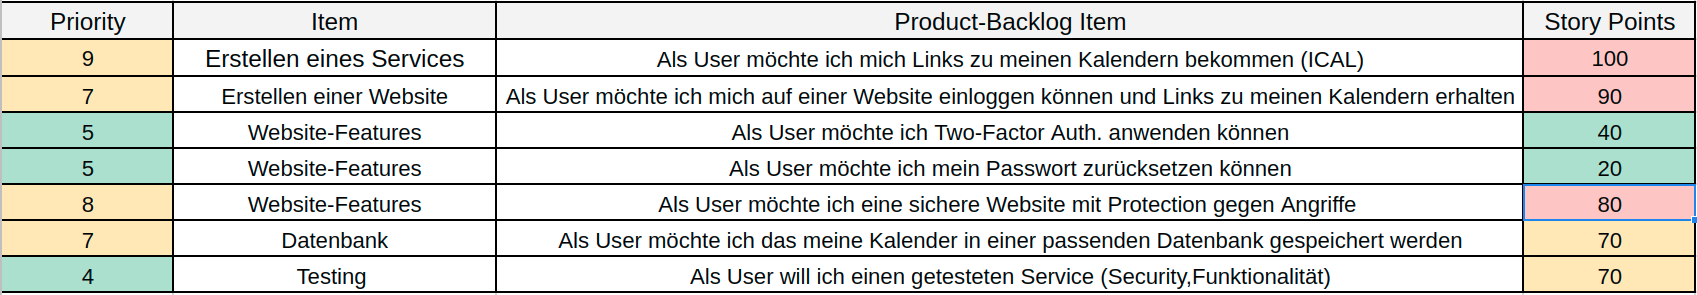
\includegraphics[width=\textwidth]{ProjektmanagementUndOrganisation_ProductBacklog.png}
    \caption{Product-Backlog}
    \label{fig:productBacklog}
\end{figure}
				
			\textbf{Product-Increment} \\
			Das Ziel von Scrum ist es, nach jedem Sprint ein potenziell veröffentlichbares Produkt vorzeigen zu können. Dieses Produkt muss getestet, fertig und von hoher Qualität sein. Ein Beispiel wäre, dass nach einem Sprint ein Benutzer sich anmelden können soll, dies bedeutet aber nicht das der Benutzer sich auch abmelden können muss. Somit muss nach einem Sprint ein fertiges und funktionierendes Stück Software vorweisbar sein, das heißt allerdings nicht, dass andere Funktionen welche mit der Funktion welche in diesem Sprint implementiert wurde zusammenhängen auch fertiggestellt werden müssen. Das Product-Increment ist kein Dokument sondern Code welcher nach jedem Sprint fertig und funktionstüchtig sein muss. \textcite{ScrumProduct-Increment}\\

			\textbf{Sprint-Backlog} \\ 
			Vor jedem Sprint gibt es ein Sprint-Planning Meeting welches in \ref{sec:Rollen} erklärt wird. In diesem Meeting wird der Sprint-Backlog angefertigt. Der Sprint-Backlog beinhaltet Einträge aus dem Product-Backlog welche im kommenden Sprint durchgeführt werden sollen. Der Product-Owner hat das finale Entscheidungsrecht welche Product-Backlog Items letztendlich in den Sprint-Backlog gelangen. Es werden oft auch noch genauere Informationen zu den Elementen aus dem Product-Backlog hinzugefügt falls zusätzliche Informationen benötigt werden.
			Einträge im Sprint-Backlog nennt man Sprint-Backlog Tasks. Der Aufwand einzelner Sprint-Backlog Tasks wird wie beim Product-Backlog geschätzt und niedergeschrieben.
			Wie die Sprint-Backlog Tasks abgearbeitet werden bestimmt das Team welches in \ref{sec:Rollen} beschrieben wird. Das Team hat auch die Aufgabe den Sprint-Backlog zu pflegen indem der Status von Sprint-Backlog Tasks verändert wird. Wenn ein Eintrag gerade durchgeführt wird, ist er "in Arbeit", fertige Tasks werden mit "Fertig" markiert, und Einträge welche noch nicht in bearbeitung sind werden mit "offen" markiert um den Sprint-Backlog übersichtlich zu gestalten. Diese Benennungen sind aber dem Team selbst überlassen sollten allerdings nicht weggelassen werden.\textcite{ScrumSprint-Backlog} \\ 
			
\begin{figure}[H]
	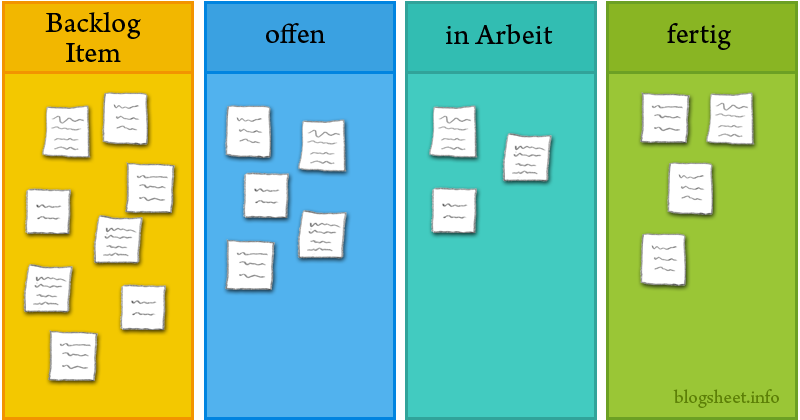
\includegraphics[width=\textwidth]{ProjektmanagementUndOrganisation_SprintBacklog.png}
    \caption{Sprint-Backlog}
    \label{fig:sprintBacklog}
\end{figure}
		
	\paragraph{Rollen}
	\label{sec:Rollen}
		Bei Scrum wird das Team in Rollen eingeteilt, jede Rolle hat eine spezielle Funktionalität welche im Laufe des Projekts durchgeführt werden muss. Eingeteilt wird in Product Owner, Scrum-Master und das Team. \\

			\textbf{Product Owner} \\
			Der Product Owner oder kurz PO ist essenziell für eine erfolgreiche Durchführung von Scrum. Der PO ist kein Komitee, sondern immer nur eine Person, auch wenn der PO kein Komitee ist kann er oder sie ein Komitee vertreten. Der Product-Backlog wird vom PO erstellt und der PO muss sicherstellen, dass das Team jeden Eintrag im Product-Backlog versteht, genaueres zum Product-Backlog im Kapitel \ref{sec:Artefakte}. Die wichtigste Aufgabe des Product-Owners ist die Verbesserung der Effizienz des Teams. Dies kann erreicht werden indem Product-Backlog Items ordentlich Priorisiert werden und der PO mit Stakeholdern kommuniziert und diese über die aktuellen Ergebnisse informiert. Weiters ist der PO für die Leistungskontrolle zuständig, er oder sie erklärt Product-Backlog Items für fertig oder nicht. \textcite{ScrumProductOwner} \\ 
			
			\textbf{Scrum-Master} \\
			Die Hauptaufgabe des Scrum-Masters ist es, sicherzustellen, dass der Scrum-Prozess ordentlich durchgeführt wird indem er oder sie Konflikte im Team stillt, einen Blick auf die Artefakte hat und beseitigt Hindernisse welche sich im Entwicklungszyklus aufgeben können. Der Scrum-Master ist die Kommunikationsschnittstelle zwischen dem Team und dem Product-Owner welche beide im Kapitel \ref{sec:Rollen} näher behandelt werden. Weiters moderiert ein Scrum-Master Meetings welche im Scrum-Prozess anfallen. Der Scrum-Master ist allerdings nicht der Projektleiter, er oder sie befasst sich mit dem Scrumablauf und nicht damit wie einzelne   Funktionalitäten implementiert werden. Ein Scrum-Master welcher gleichzeitig Teammitglied oder Product-Owner ist kann zu Interessenskonflikten führen, sollte somit also vermieden werden. \textcite{ScrumScrumMaster} \\
			
			\textbf{Team} \\
			In einem Scrum-Prozess gibt es 2 Teams, das Team im allgemeinen welches aus Product-Owner, Scrum-Master und dem Entwicklungsteam besteht, und das Entwicklungsteam im einzelnen. Dieses Kapitel wird sich mit dem Entwicklungsteam befassen. Die Aufgabe des Entwicklungsteams ist es am Ende eines Sprints ein potenziell lieferbares Product-Increment fertiggestellt zu haben, eine Erklärung zum Product-Increment ist im Kapitel \ref{sec:Artefakte}. Entwicklungsteams sind selbstorganisierend, das heißt, dass niemand dem Entwicklungsteam vorschreiben kann wie sie etwas zu machen haben.
			Die größte des Teams spielt eine wichtige Rolle in der Produktivität. In einem kleinen Team wird es nur selten zu Kommunikationsproblemen kommen aber es ist schwierig mit einem kleinen Team alle Kenntnisse welche für ein Projekt benötigt werden abzudecken. Ein zu großes Team vergrößert den Organisatorischen Aufwand enorm und ist somit trotz wahrscheinlicher Abdeckung aller benötigten Kenntnisse nicht wünschenswerte Ergebnisse erbringen. Ein Team von 4 - 6 Entwicklern und Entwicklerinnen ist nur selten falsch. \textcite{ScrumTeam} \\
			
		
	\paragraph{Meetings}
	\label{sec:Meetings}
		Meetings sind ein extrem wichtiger Teil des Scrumprozesses, solange sie gut geleitet werden und von jedem Teammitglied ernst genommen werden können sie die Effizienz enorm steigern. Essentielle Ereignisse sind das Sprint-Planning-meeting, der Daily-Scrum, die Sprint-Retroperspective und der Sprint-Review. 
